\documentclass{article}

\usepackage{tabularx}
\usepackage{booktabs}
\usepackage{graphicx}
\usepackage{paralist}
\usepackage{listings}
\usepackage{booktabs}
\usepackage{hyperref}
\usepackage{amsfonts}
\usepackage{amsmath}
\usepackage{color}
\usepackage{fancyhdr}
\usepackage{geometry}
\usepackage{soul}
\usepackage{multirow}
\usepackage{ulem}
\usepackage{float}
\usepackage{tikz}



\title{SRS\\Digital Twin Forest}
\author{Yichen Jiang, Bowen Zhang, Jiacheng Wu, Junhong Chen, Tingyu Shi\\Team 8}

\begin{document}

\maketitle
%%%%%%%%%%%%%%%%%%%%%%%% Revision History %%%%%%%%%%%%%%%%%%%%%%%%%%%%%%%
\newpage
\begin{table}[htp]
\caption{Revision History} 
\begin{tabularx}{\textwidth}{llX}
\toprule
\textbf{Date} & \textbf{Developer(s)} & \textbf{Change}\\
\midrule
Sept 24, 2022 & All team members & Initial Document\\
\hline
Sept 26, 2022 & All team members & Update Requirements\\
\hline
Sept 29, 2022 & All team members & Revision 0\\
\hline
March 29, 2023 & All team members & Final Version\\
\bottomrule
\end{tabularx}
\end{table}
%%%%%%%%%%%%%%%%%%%%%%%%%%%%%%%%%%%%%%%%%%%%%%%%%%%%%%%%%

\vspace{5cm}

%%%%%%%%%%%% Template Information %%%%%%%%%%%%%%%%%%%%%%%%%%%%%%%
\noindent This document follows \href{https://www.cs.uic.edu/~i440/VolereMaterials/templateArchive16/c\%20Volere\%20template16.pdf}{\textcolor{red}{Volere Template}}.
The following are some modifications that we made to the 
original template:
\begin{itemize}
    \item We added traceability matrices to show relationships between
    functional requirements and non-functional requirements.
    \item We added traceability matrices to show relationships between requirements and 
    use cases.
    \item We added Likely changes and Unlikely changes.
    \item We added priorities and 
    completion timelines for each functional requirement.
\end{itemize}

%%%%%%%%%%%%% Template Information End %%%%%%%%%%%%%%%%%%%%%%%%%%%%

\newpage

%%%%%%%%%%%%%%Contents%%%%%%%%%%%%%%%%
\tableofcontents
\listoftables
\listoffigures
\cleardoublepage

%%%%%%%%%%% Project Drivers %%%%%%%%%%%%
\section{Project Drivers}
\subsection{The purpose of the Project}
\subsubsection{The User Business or Background of the Project Effect}
A digital twin is a virtual representation of the real
forest located at Turkey Point, Ontario, it includes physical objects, 
processes, relationships, and behaviors. Elements of a digital twin
include data capture and integration, visualization,
advanced analysis including AI, automation, and information
sharing and collaboration. This project can be beneficial
for two groups of users.  The first group of users is forest owners. 
This project can help them to manage the forest. The second group of users is
meteorologists. This project can help them to do research. 

\subsubsection{Goals of the Project}
\begin{itemize}
\item A virtual representation of the real forest,
allowing monitoring and analyzing from distance.
\item Visualizing important data related to scientific 
research and decision-making. For the environment, 
important data include temperature, humidity, etc. 
For tree parameters, important data include tree density,
tree heights, tree diameters, etc.
\item A forest model that can change dynamically 
according to the modification of the data.
\end{itemize}

\subsection{Stakeholders}
\subsubsection{The client}
\begin{itemize}
\item Dr. Alemu Gonsamo from School of Earth,
    Environment and Society McMaster University (Dr.
    Gonsamo is the supervisor of this project.)
 
\end{itemize}
\subsubsection{The Customer}
\begin{itemize}
    \item Forest Owners(The final project can be helpful for forest owners to better manage the 
    forest and make decisions)
    \item Meteorologists(The final product can be helpful for researchers to 
    study climate change)
\end{itemize}

\subsubsection{Other Stakeholders}
\begin{itemize}
    \item Dr. Gonsamo's lab members(Graduate students from the lab will provide suggestions and
    data needed to assist this project)
\end{itemize}

\subsubsection{The Hands-On Users of the Product}
The hands-on users of this product are the same as the customers mentioned in section 1.2.2. Users'
responsibilities are also mentioned in section 1.2.2. For subject matter experience, these 
users are masters. For both forest owners and meteorologists, they are definitely
familiar with the real forest and our product can help them better do
their jobs. From the point of technology, we assume that they 
have little experience with virtual representation
technologies.

\subsubsection{Personas}
\begin{itemize}
    \item Dr. Aly is a 55-year-old assistant professor working in a university, living with his family near his lab. His research mainly focuses on remote sensing of vegetation, global change ecology, and climate change impact. His research is supported by an association of several forest owners, who are willing to let Dr. Aly locate part of the research and collect needed information in their forest. If he needs to go to the field that day, the typical schedule of him is to get up at 6 am, take 90 minutes to commute to the target forest with some students he supervises, collect and record data there, and come back to his lab with another 90 minutes. 
    
    Dr. Aly's goals are to find a convenient way to free him from frequent commuting and to look for a new method to manage and visualize all the significant data for a purpose of teaching. 
    
    \item Mrs. Miller owns 40-acre land including a 2-acre forest. She is now 36 years old and lives with her husband, who works as a financial analyzer, in Toronto. She runs a coffee house as a full-time job and drives to her forest every two months to check everything's fine. Though she cares about her forest, spending over three days every two months going through every area seems impossible for her, she would love to have a new method to manage her forest and get updated information regularly, in order to make better strategies for the forest. 
\end{itemize}

\subsubsection{Priorities Assigned to Users}
\begin{itemize}
    \item Key Users: Dr. Gonsamo, Forest owners, meteorologist
    \item Secondary Users: Lab members
\end{itemize}

\subsubsection{User Participation}
\begin{itemize}
    \item Dr. Gonsamo: Dr. Gonsamo will provide business knowledge(forest data), 
    interface prototyping and usability requirements for this project. Since Dr. Gonsamo is 
    a meteorologist, he can also provide suggestions for meteorologists.
    \item Lab members: Lab members will help this project by providing some business knowledge
    about the forest.
    \item Forest Owners: Forest owners can provide commercial data about the forest. Commercial
    data include tree-cutting data, annual profits, etc.
\end{itemize}
\subsubsection{Maintenance Users and Service Technicians}
The project members will be responsible for maintaining and changing the product.
%%%%%%%%%%% Project Drivers End %%%%%%%%%%

\newpage

%%%%%%%%%% Project Constraints %%%%%%%%%%%%
\section{Project Constraints}
\subsection{Mandated Constraints}
\subsubsection{Solution Constraints}
\begin{itemize}
\item Modeling Technology: Our team will use Unity for
the modeling task. The Unity version will be 2021.3. Our
team members use different platforms(Windows or MacOS).
Unity is suitable for our team because it is a 
cross-platform software. Also, Unity has existing
packages that can speed up our modeling process.
    
\item Project Documents Technology: Our team will use
\LaTeX for our documents.
    
\item Project Cooperation Technology: Our team will use
GitHub to cooperate.
\end{itemize}

\subsubsection{Implementation Environment of the Current System}
The product will be installed on Windows and MacOS 
operating systems.

\subsubsection{Partner or Collaborative Applications}
N/A(Our product is an independent product)

\subsubsection{Off-the-Shelf Software}
\begin{itemize}
\item LiDAR: iPad Pro LiDAR should be used to scan the
forest and collect data for modeling.
\item Unity: Unity should be used for modeling and 
post-processing.
\item ArcGIS: An online tool to visualize forest 
distribution and tree data. The team can calculate the
the density of different tree species and the formulas 
according to the tree distribution based on the
satellite pictures.
\end{itemize}

\subsubsection{Anticipated Workplace Environment}
Both indoor and outdoor are possible workplace environments. 

\subsubsection{Schedule Constraints}
Please check our project schedule \href{https://github.com/wuj187/DigitalTwinCAS/tree/main/docs/DevelopmentPlan/Project_Schedule}{\textcolor{red}{here}}. The following are known
deadlines:
\begin{itemize}
\item SRS Rev0 (October 5)
\item Hazard Analysis 0 (October 19)
\item V\&V Plan Rev0 (November 2)
\item POC Demo (November 14)
\item Design Document Rev0 (January 18)
\item Demonstration Rev0 (February 14)
\item V\&V Report Rev0  (March 8)
\item Final Demo (April 1)
\item Final Documentation (April 5)
\end{itemize}

\subsubsection{Budget Constraints}
Total expenses should not exceed \$750.

\subsubsection{Enterprise Constraints}
N/A This project is not invested by any enterprise.

\subsection{Naming Conventions and Definitions}
\begin{itemize}
    \item LiDAR: Light Detection and Ranging(Scanning Technology)
    \item Plot: A square-shaped area in the forest. There are 14 plots in total. 
    \item LAI: Leaf Area Index
    \item DBH: Diameter at Breast Height
    \item Target Forest: Target forest refers to the natural forest located at Turkey
    Point in Ontario.
    \item Digital Twin Forest: The virtual representation of the target forest.
    \item Forest Data: Forest Data include environmental data and tree parameters.
    \item Environmental Data:
    \begin{itemize}
        \item Humidity
        \item Temperature
        \item Soil Carbon Content
        \item Soil Nitrogen Content
        \item LAI 
    \end{itemize}
    \item Tree parameters: 
    \begin{itemize}
        \item Density
        \item Height
        \item Age
        \item DBH 
    \end{itemize}
    \item Tree types. There are 7 different types of trees,
    the following are the details:
    \begin{itemize}
        \item Red Pine
        \item Oak
        \item Birch 
        \item Beech
        \item White Pine
        \item Red Maple
        \item Red Oak
    \end{itemize}
\end{itemize}

\subsection{Relevant Facts and Assumptions}
\subsubsection{Relevant Facts}
\begin{itemize}
    \item Forest data keep changing all the time, but our 
    system will only update weekly. Therefore, the 
    system may not be able to reflect the most accurate data. 
    However, since the forest data will not change dramatically
    within a short period of time, the system should be 
    close to the real forest.
    \item The product can be beneficial for meteorologists to do research.
    \item The product can be beneficial for forest owners 
    to better manage the forest.
\end{itemize}

\subsubsection{Business Rules}
N/A

\subsubsection{Assumptions}
\begin{itemize}
    \item Unity and required toolboxes 
    should be accessible to all developers'
    devices.
    \item Users will use our product on Windows and MacOS.
    \item Forest data will not change dramatically within a 
    short period of time. 
    \item Related data to the forest shown in the product will be manually updated by the users.
\end{itemize}
%%%%%%%%%%%% Project Constraints End %%%%%%%%%

\newpage

%%%%%%%%%%% Functional Requirements %%%%%%%%%%%%
\section{Functional Requirements}
\subsection{The Scope of the Work}
\subsubsection{The Current Situation}
Currently, digital twin technologies are being utilized in many
areas, such as Aerospace and Aeronautics, manufacturing, automotive, etc. For more 
detailed information, please check paper \href{https://github.com/wuj187/DigitalTwinCAS/blob/main/refs/DT_Applications.pdf}{\textcolor{red}{\textit{Applications of Digital Twin across 
Industries: A Review}}} in our reference folder. This paper talks about 
many applications of digital twin technologies in different areas.\\
The following is the reference of the above paper:\\
Singh, M., Srivastava, R., Fuenmayor, E., Kuts, V., Qiao, Y., Murray, N., 
\& Devine, D. (2022). Applications of Digital Twin across industries: a 
review. \textit{Applied Sciences}, 12(11), 5727.\\

\noindent
After searching online, we found a similar product from Tietoery
Company called \href{https://www.tietoevry.com/en/industries/forest-pulp-paper-and-fibre/forest-solutions/wood-and-fibre-ecosystem-and-integration/digital-forest-twin/}{\textcolor{red}{Digital Forest Twin}}.
According to its introduction, this product can 
be accessed using head-mounted devices or
web browsers, which is different from our product. Also, 
from the company's website, we can know little details about how
 this product works. Therefore, our team does not know too much
 about existing business processes.

 \newpage
 
\subsubsection{The Context of the Work}
The following is the context of the work diagram:
\begin{figure}[H]
\begin{center}
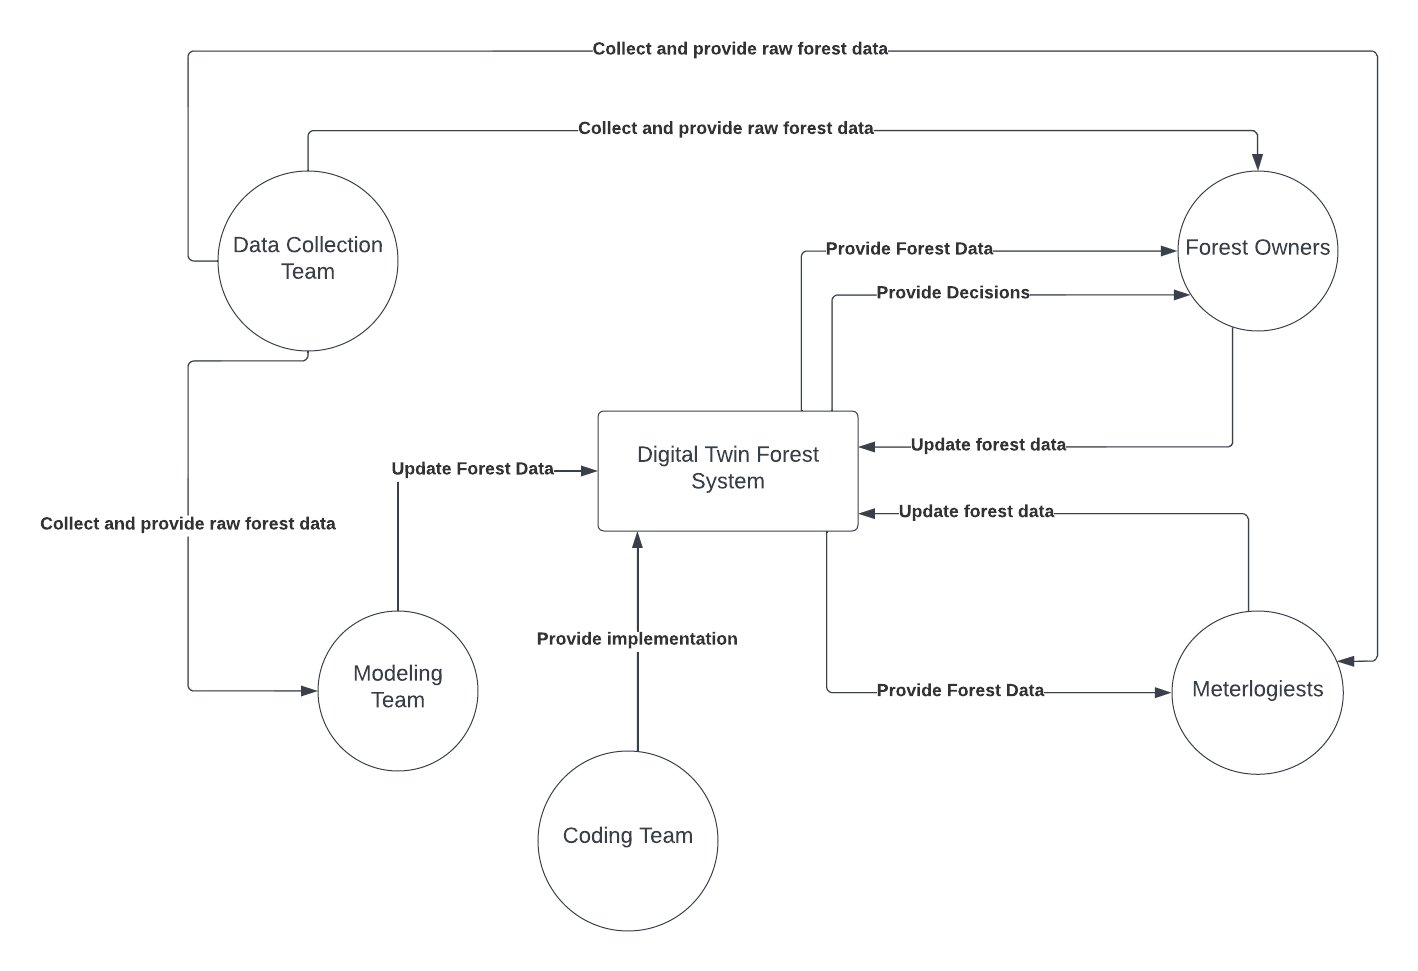
\includegraphics[scale=0.7]{SRS_Pictures/Context_Use.png}
\end{center}
\caption{Context of the Work Diagram}
\end{figure}

\noindent Forest data include the following:
\begin{itemize}
\item Environmental Data:
\begin{itemize}
    \item Humidity
    \item Temperature
    \item Soil Carbon Contents
    \item Soil Nitrogen Contents
    \item LAI
\end{itemize}
\item Tree Parameters:
\begin{itemize}
    \item Density
    \item Age
    \item Height
    \item DBH
\end{itemize}
\end{itemize}

\subsubsection{Work Partitioning}
\begin{table}[H]
\caption{Business Event List} 
\begin{tabularx}{\textwidth}{XXX}
\toprule
\textbf{Event Name} & \textbf{Input and Output} & \textbf{Summary of BUC}\\
\midrule
Update Forest Data & Forest Data(in) & After the system receives new data, it 
should store the data in the Data Store.\\
\hline
Data visualization & Forest Data(output) & The system demonstrates the organized 
forest data to the users. The data presented should be consistent with 
the data in the Data Store.\\
\hline
Model Demonstrations & Forest Models(output) & The system demonstrates the 
forest models to the users. The models presented should be generated according 
to the data stored in the Data Store\\
\bottomrule
\end{tabularx}
\end{table}

\newpage

\subsubsection{Specifying a Business Use Case (BUC)}
The following is an activity diagram for the Data Visualization process.
\begin{figure}[H]
    \centering
    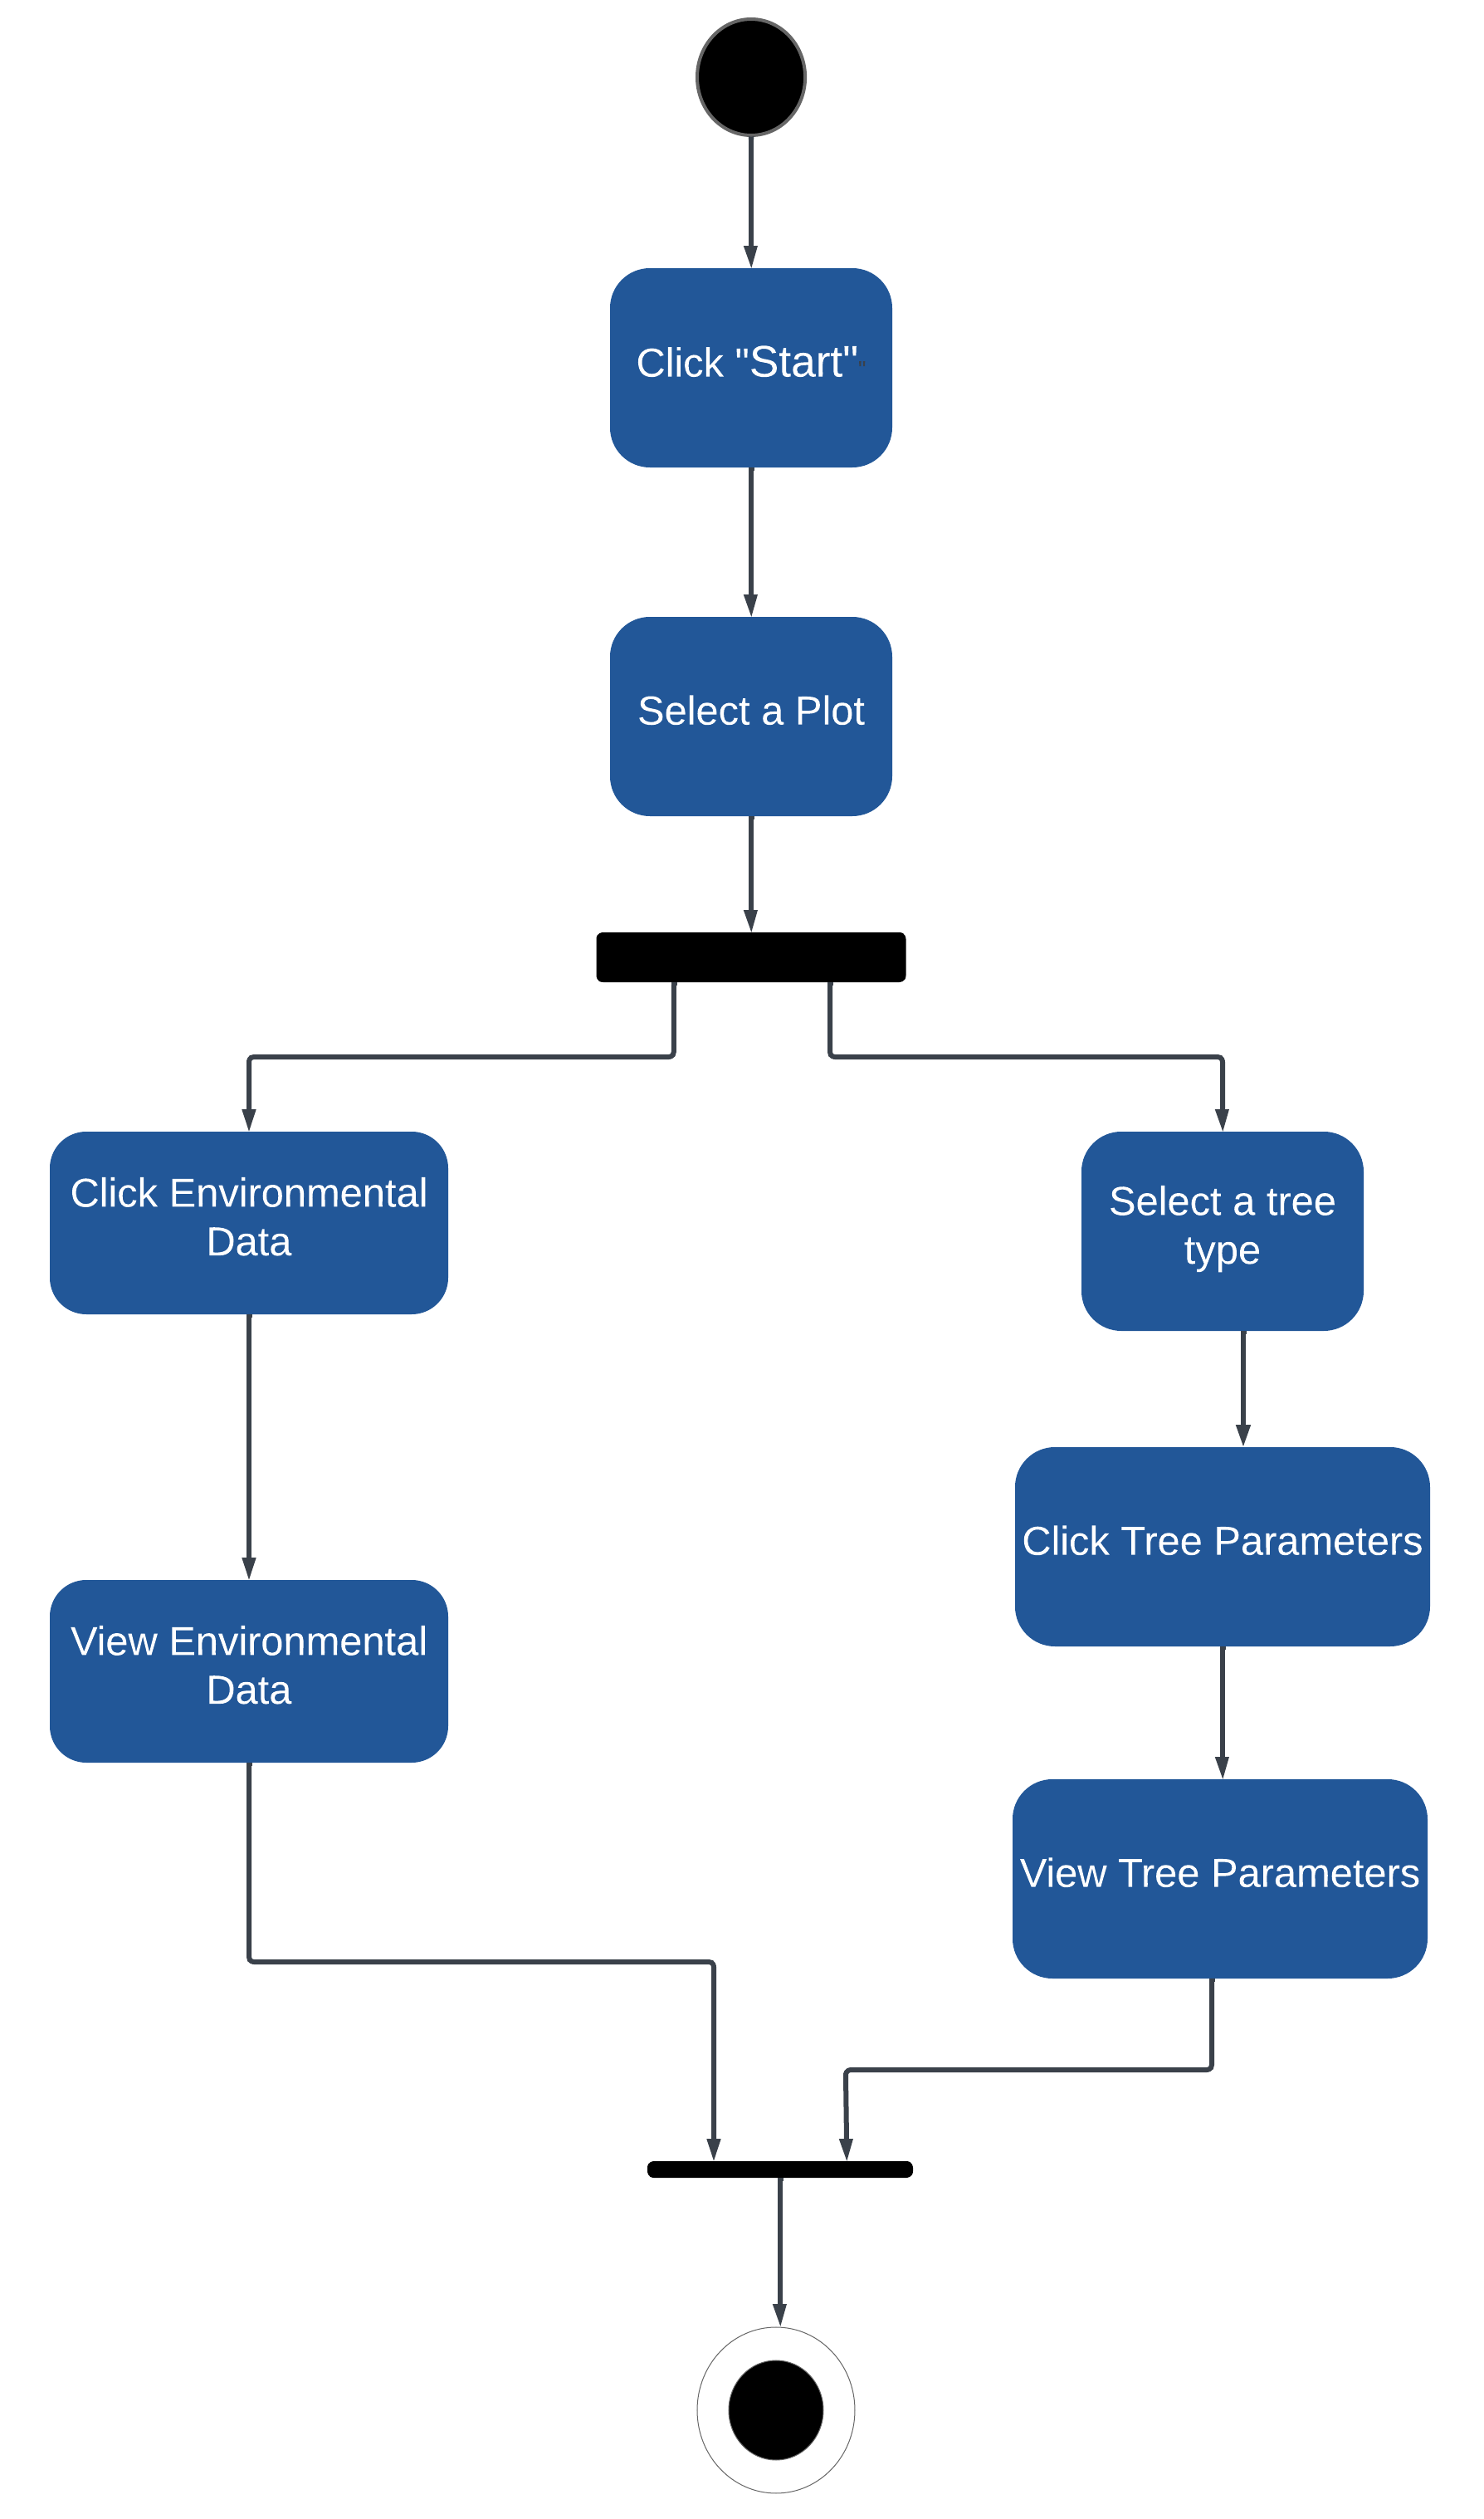
\includegraphics[scale=0.35]{SRS_Pictures/Activity_Diagram.png}
    \caption{An activity diagram for the Data Visualization process}
\end{figure}

\subsection{Business Data Model and Data Dictionary}
The following picture shows the forest data hierarchy:
\begin{figure}[H]
    \centering
    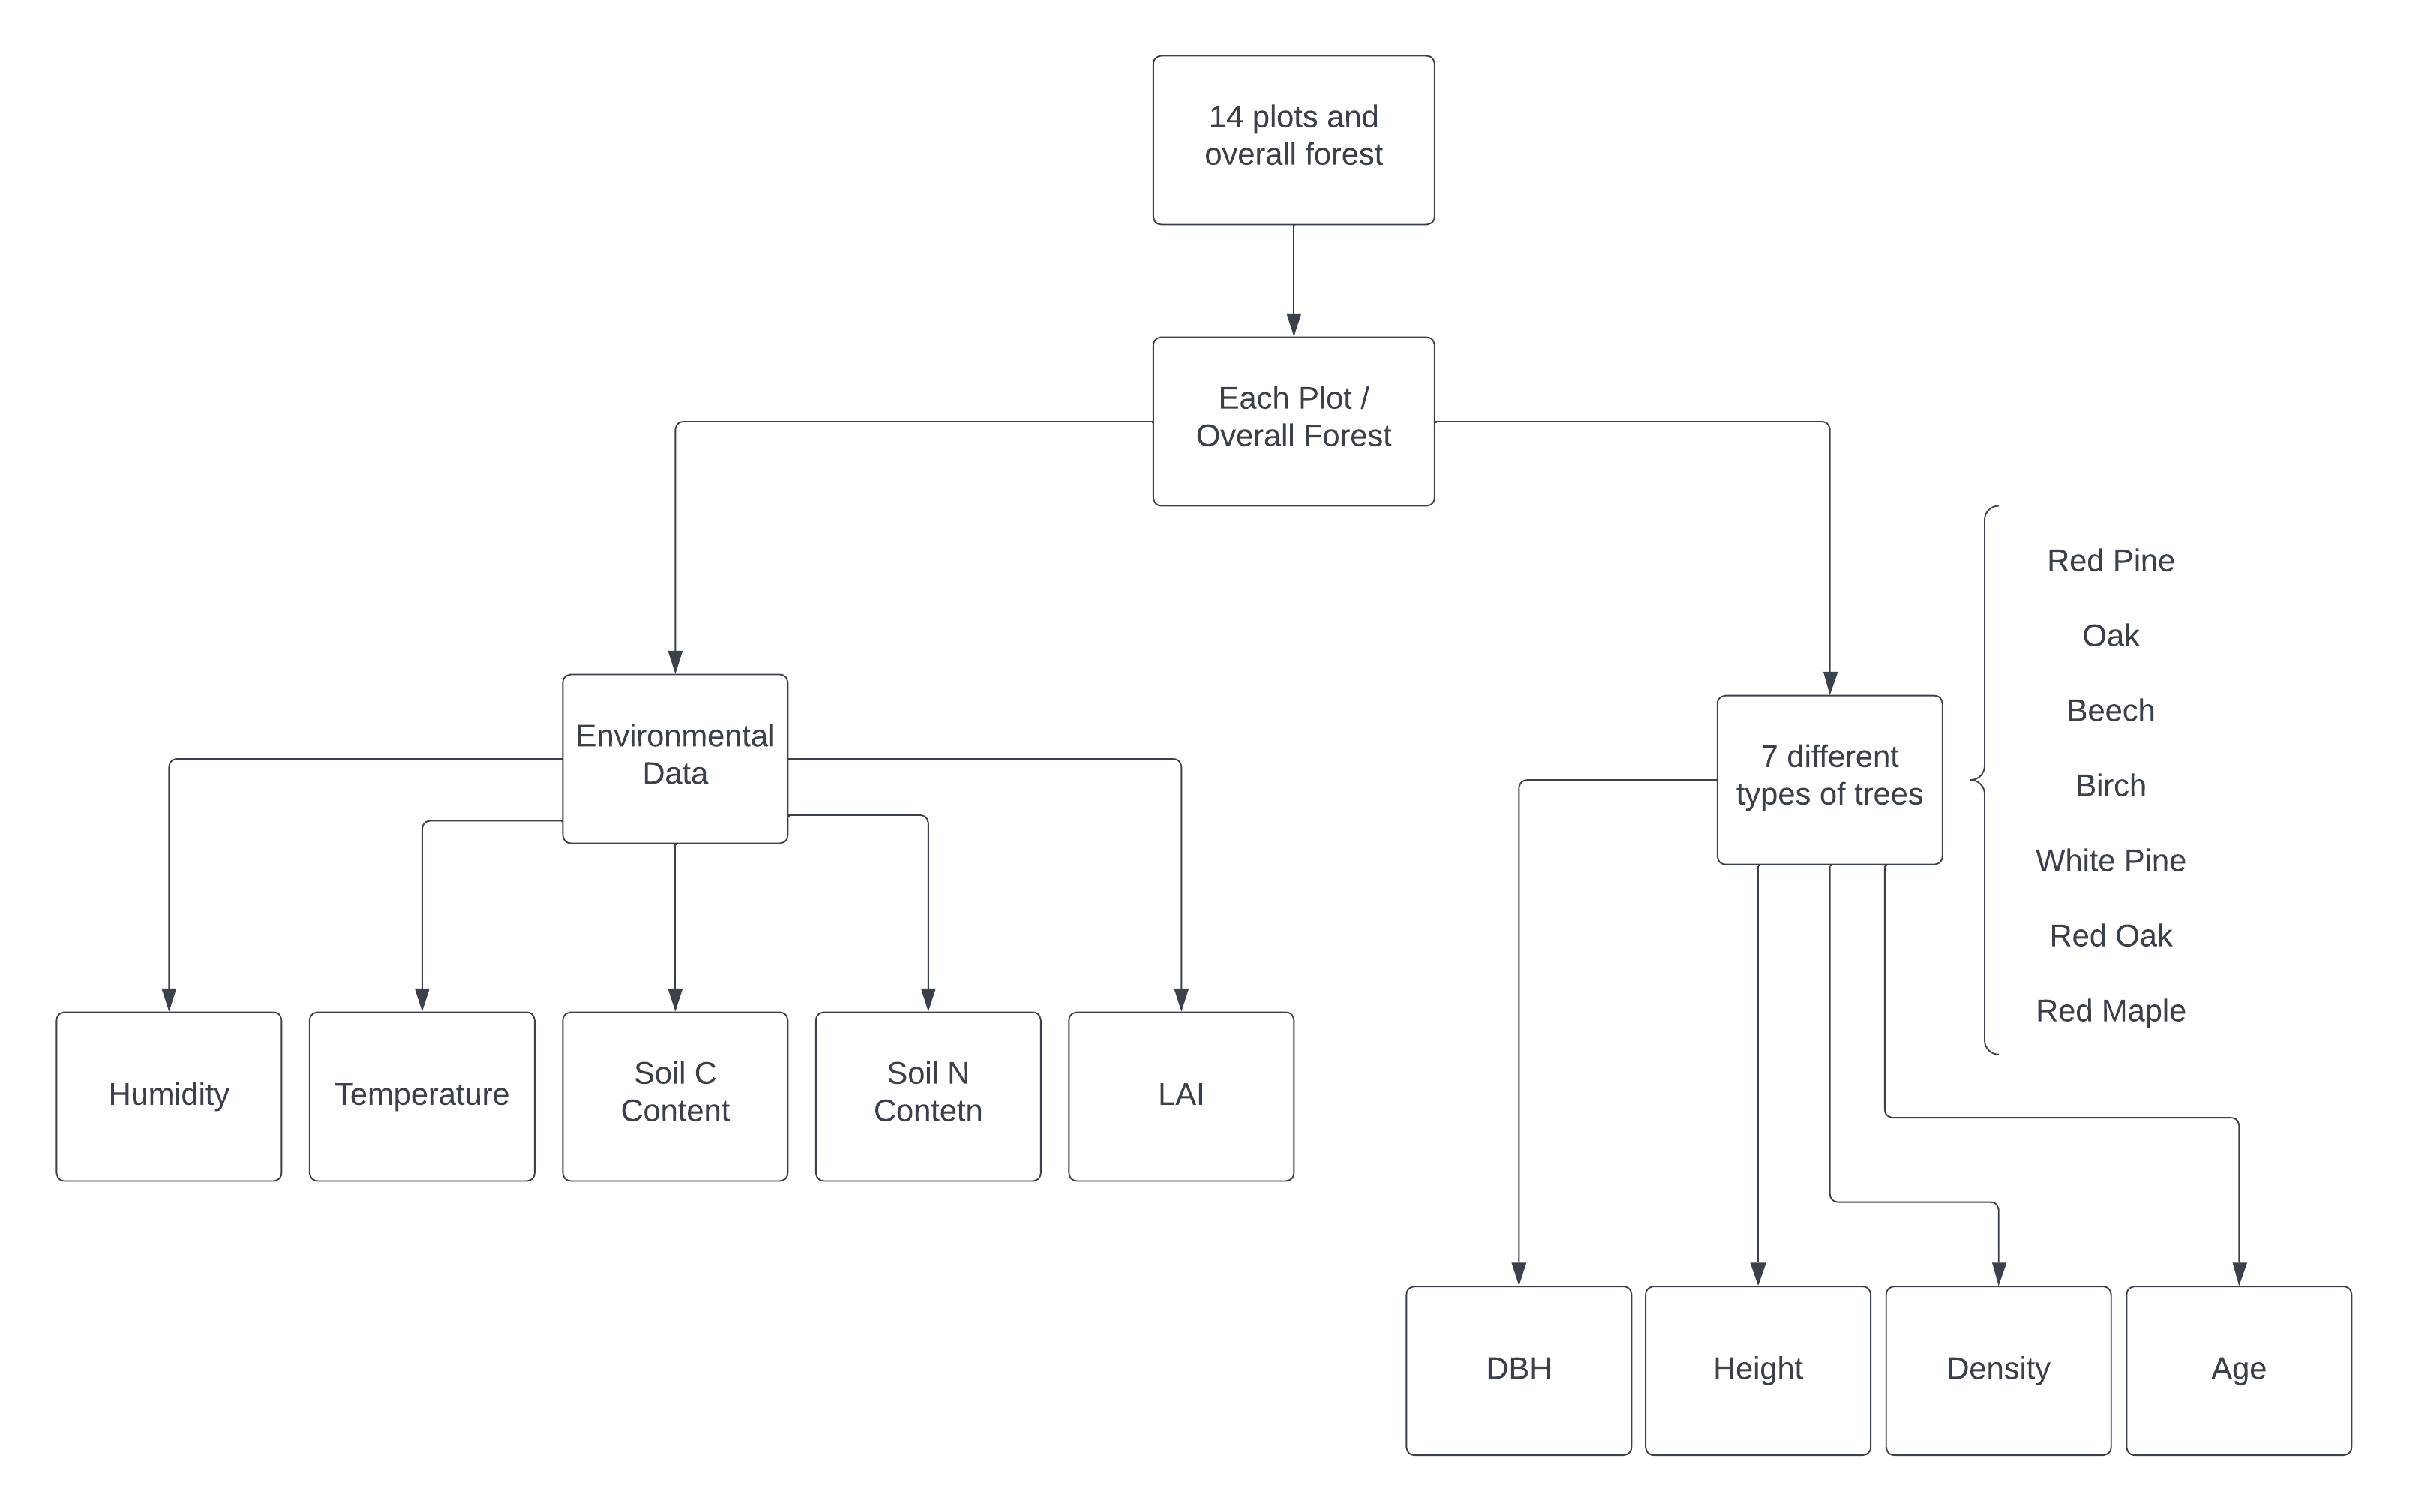
\includegraphics[scale = 0.65]{SRS_Pictures/Data-Hierchary.png}
    \caption{Data Hierarchy}
\end{figure}

\newpage

\subsection{The Scope of the Product}
\subsubsection{Product Boundary}
\begin{figure}[H]
    \centering
    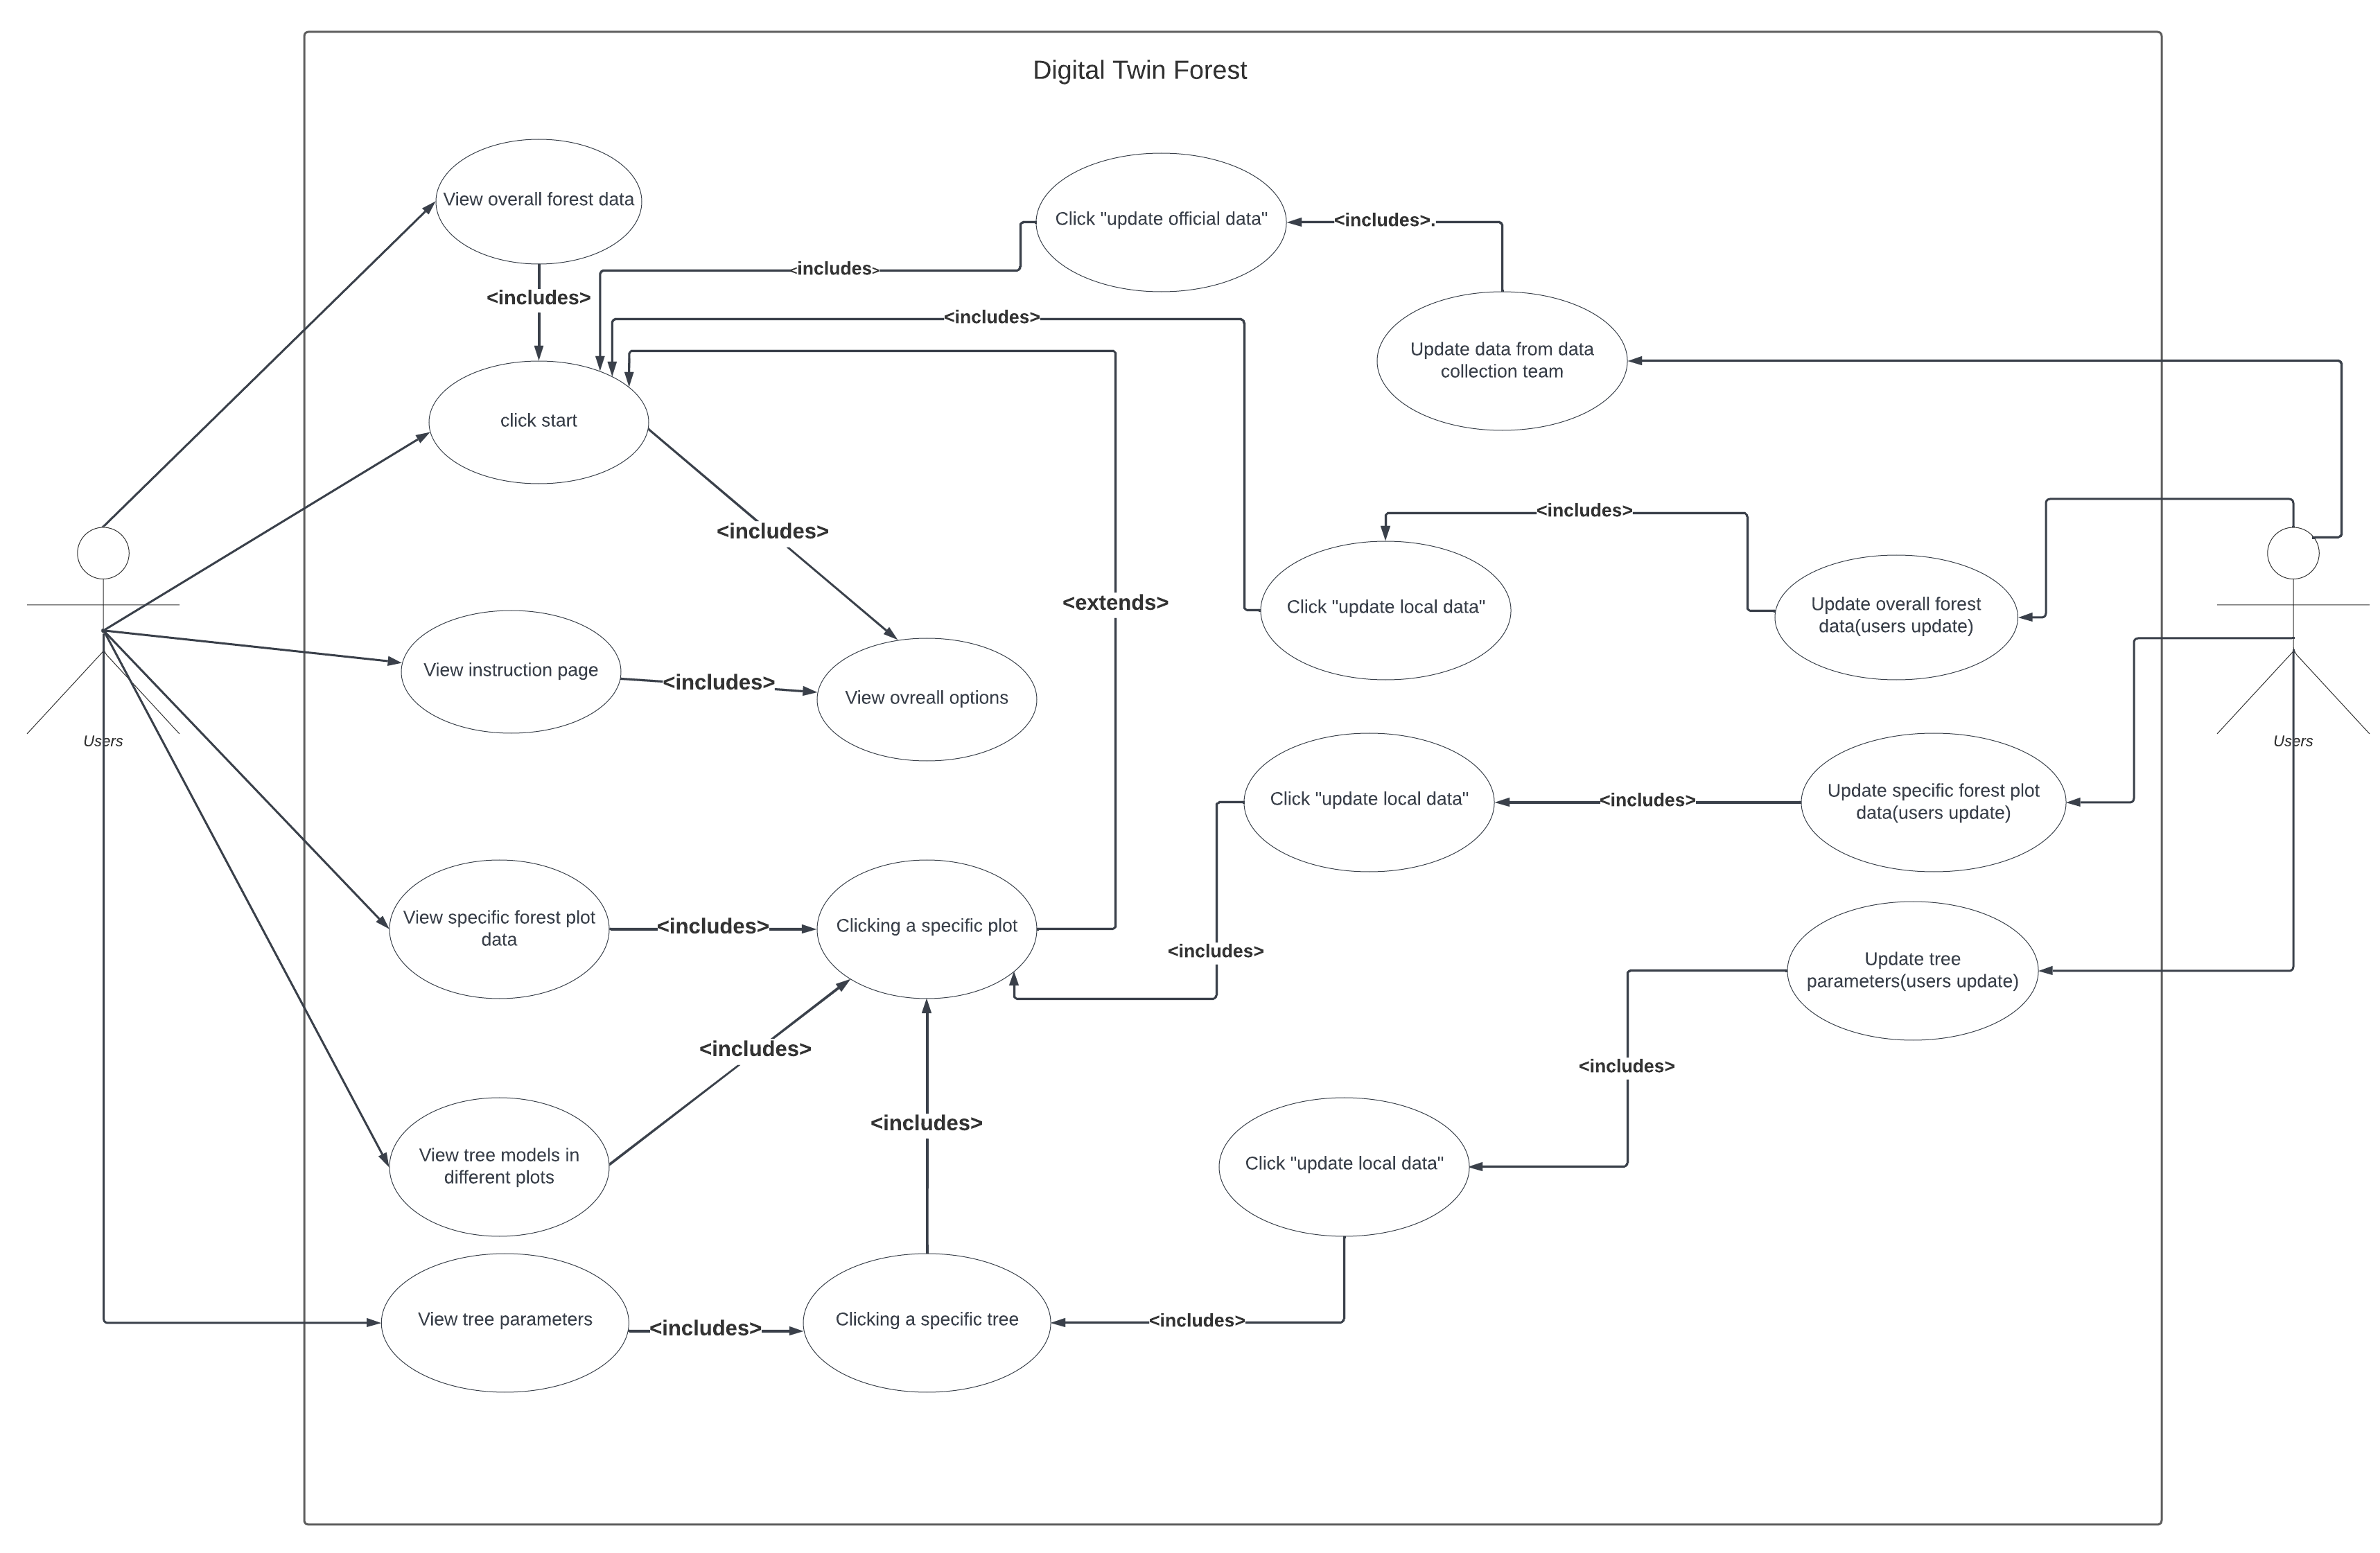
\includegraphics[scale=0.28]{SRS_Pictures/Use_Case.png}
    \caption{Use Case Diagram}
    \label{usecase}
\end{figure}


\subsubsection{Product Use Case Table}
\begin{enumerate}
\item PUC Name: View instructions\\
Actor: Users\\
Input: Users click \verb|Instruction| button at the beginning of the
application.\\
Output: Application instructions should appear on the screen. 

\item PUC Name: View group member information\\
Actor: Users\\
Input: Users click \verb|Contact Us| at the beginning of the application.\\
Output: Group members' contact information should appear on the screen.

\item PUC Name: Update Data\\
Actor: Users\\
Input: This use case involves many actions. Please check Figure \ref{usecase}.\\
Output: Newly entered data should be stored in Data Store successfully. 

\item PUC Name: View  forest  data\\
Actor: Users\\
Input: This use case involves many actions. Please check Figure \ref{usecase}.\\
Output: Environmental data or tree parameters should appear on the screen.

\item PUC Name: View forest models\\
Actor: Users\\
Input: This use case involves many actions. Please check Figure \ref{usecase}.\\
Output: Forest models appear on the screen.

\item PUC Name: Quit software\\
Actor: Users\\
Input: Click \verb|Quit| button.\\
Output: Software should quit successfully.

\end{enumerate}



\subsection{Functional Requirements}

\begin{enumerate}[FR1]
\item The product shall provide an option to display basic
instructions.\\
\textbf{Rationale}: Users might not be familiar with our
product, especially when they use it for the first time.\\
\textbf{Fit Criterion}: A basic instruction option shows up
on the user interface after the software is launched. \\
\textbf{Supporting Materials}: All requirements using the instruction page.\\
\textbf{Dependencies}: N/A\\

\item The product shall provide an option to display the contact information of
the development team.\\
\textbf{Rationale}: Users may want to contact us when they have questions about the product.\\
\textbf{Fit Criterion}: A contact-us page shows up
on the user interface after the software is launched. \\
\textbf{Supporting Materials}: All requirements using the contact us page.\\
\textbf{Dependencies}: N/A\\
	
\item The product shall load the forest model when users access the model
page.\\
\textbf{Rationale}: The clicking of `start' indicates the
user has been through the instruction and is ready to use
our product. The product can now initialize the functions
by loading the model.\\
\textbf{Fit Criterion}: The software loads the data and 
models of the forest once the users select the `start' 
button.\\
\textbf{Supporting Materials}: All requirements using the forest model.\\
\textbf{Dependencies}: N/A\\


\item The product shall allow users to minimize the user
interface. (User interface includes windows that present
forest data). \\
\textbf{Rationale}: The user might want to pay more 
attention to the model instead of information related to
it. Minimizing the user interface allows the user to do so. \\
\textbf{Fit Criterion}: The windows of the user interface
will be minimized to the side of the screen once the user
clicks the \textit{minimized} button on the user interface.\\
\textbf{Supporting Materials}: All requirements interacting with the panel of forest data.\\
\textbf{Dependencies}: N/A\\

\item The product shall be able to display 
environmental data when users select a specific forest plot.\\
\textbf{Rationale}: Environmental data are very essential for the real forest.
Therefore, we need a way to visualize environmental data in our product.\\
\textbf{Fit Criterion}: Users can check environmental data successfully from
the User Interface.\\
\textbf{Supporting Materials}: All requirements using the environmental data.\\
\textbf{Dependencies}: N/A\\

\item The product shall be able to display tree parameters
when users select a specific tree type.\\
\textbf{Rationale}: Tree parameters are very essential for the real forest.
Therefore, we need a way to visualize tree parameters in our product.\\
\textbf{Fit Criterion}: Users can check tree parameters successfully from
the User Interface.\\
\textbf{Supporting Materials}: All requirements using the tree parameters.\\
\textbf{Dependencies}: N/A\\

\item The product shall display the forest data 
 without interrupting users viewing forest models.\\
\textbf{Rationale}: The product should display the important data that our users
might care about on the user interface while not letting the information interrupt
the display of the model. Therefore, it should distribute the information on both
sides.\\
\textbf{Fit Criterion}: When the full view of the forest is displayed, windows 
containing the overall information about the forest shall be shown on both sides
of the screen. \\
\textbf{Supporting Materials}: All requirements asking for usability.\\
\textbf{Dependencies}: N/A\\

\item The product shall allow users to move around within the forest.\\
\textbf{Rationale}: The user might want to see different perspectives of the 
forest. \\
\textbf{Fit Criterion}: When users press W, S, A, and D keys on the keyboard, the 
camera moves forward, backward, leftward, and rightward accordingly.  \\
\textbf{Supporting Materials}: All requirements related to performance.\\
\textbf{Dependencies}: N/A\\
	
\item The product shall allow users to change their perspectives. \\
\textbf{Rationale}: Users might need to observe the forest from different 
perspectives.\\
\textbf{Fit Criterion}: The user's perspective changes when he or she moves the
mouse.\\
\textbf{Supporting Materials}: All requirements related to performance.\\
\textbf{Dependencies}: N/A\\
	
\item  The product shall provide a way to present all the data when
the amount of data does not fit on one page.\\
\textbf{Rationale}: The amount of information might not fit on a single page.
Instead of compromising the user interface and minimizing the font size, 
displaying the information on several pages would be a better choice.\\
\textbf{Fit Criterion}: Several pages will show up when showing information with
very long content.\\
\textbf{Supporting Materials}: All requirements interacting with panels of forest data.\\
\textbf{Dependencies}: N/A\\
	
\item The product shall provide ways to allow users to quit the product.\\
\textbf{Rationale}: The user would need a clear signal to exit.\\
\textbf{Fit Criterion}: Once the user clicks on the 'exit' button, the application shall quit, and the process of the software shall be terminated.\\
\textbf{Supporting Materials}: All requirements about security.\\
\textbf{Dependencies}: N/A\\
    
\item The product shall allow users to update forest data.\\
\textbf{Rationale}: In order to let the application show the latest information,
it's necessary for users to update forest data by themselves.\\
\textbf{Fit Criterion}: After the user updates the latest information, the virtual
forest shall display this latest information. \\
\textbf{Supporting Materials}: All requirements about updating and maintenance.\\
\textbf{Dependencies}: N/A\\
	
\item The tree models shall synchronize with the tree parameters.\\
\textbf{Rationale}: Tree parameters vary in different plots. The synchronization 
of tree models and tree parameters can show different models according to 
different plots, making each plot unique and realistic. \\
\textbf{Fit Criterion}: After users change a tree parameter, like tree height, the
height of the tree model will change accordingly. \\
\textbf{Supporting Materials}: All requirements asking for accuracy.\\
\textbf{Dependencies}: N/A\\

\item The tree models shall allow the users to switch between summer view and 
winter view.\\
\textbf{Rationale}: A forest has two different appearances in summer and winter. \\
\textbf{Fit Criterion}: The model's appearance will change when users click the 
button to switch seasons.\\
\textbf{Supporting Materials}: All requirements asking for realism.\\
\textbf{Dependencies}: N/A\\

\item The product shall provide a pie chart to users to indicate the proportions 
of different types of trees in each plot.\\
\textbf{Rationale}: Users might want to proportions of different types of trees in
a plot.\\
\textbf{Fit Criterion}: The information window shows a pie chart indicating the
proportions of different types of trees.. \\
\textbf{Supporting Materials}: All requirements about usability.\\
\textbf{Dependencies}: N/A\\

\item The distribution of trees in the model shall correspond to the target 
forest.\\
\textbf{Rationale}: The distributions of trees in different plots are not the same
in the actual forest.\\
\textbf{Fit Criterion}: Once users enter different plots, they will see different
distribution patterns of trees.\\
\textbf{Supporting Materials}: All requirements asking for accuracy.\\
\textbf{Dependencies}:N/A\\

\end{enumerate}

\subsection{Priority and Timeline}
\begin{table}[H]
\centering
\begin{tabular}{|lll|}
\hline
\multicolumn{3}{|l|}{Priority and Timeline}                                                                                                                                 \\ \hline
\multicolumn{1}{|l|}{\begin{tabular}[c]{@{}l@{}}Functional\\ Requirements\end{tabular}} & \multicolumn{1}{l|}{Priority}        & Timeline                                   \\ \hline
\multicolumn{1}{|l|}{FR1}                                                               & \multicolumn{1}{l|}{low priority}    & October 20th, 2022 to October 27th, 2022   \\ \hline
\multicolumn{1}{|l|}{FR2}                                                               & \multicolumn{1}{l|}{meduim priority} & October 27th, 2022 to November 3rd, 2022   \\ \hline
\multicolumn{1}{|l|}{FR3}                                                               & \multicolumn{1}{l|}{high priority}   & January 26th, 2022 to February 9th, 2023   \\ \hline
\multicolumn{1}{|l|}{FR4}                                                               & \multicolumn{1}{l|}{low priority}    & November 10th, 2022 to November 17th, 2022 \\ \hline
\multicolumn{1}{|l|}{FR5}                                                               & \multicolumn{1}{l|}{meduim priority} & December 15th, 2022 to January 12th, 2023  \\ \hline
\multicolumn{1}{|l|}{FR6}                                                               & \multicolumn{1}{l|}{low priority}    & November 24th, 2022 to December 1st, 2022  \\ \hline
\multicolumn{1}{|l|}{FR7}                                                               & \multicolumn{1}{l|}{high priority}   & February 9th 2023 to February 16th, 2023   \\ \hline
\multicolumn{1}{|l|}{FR8}                                                               & \multicolumn{1}{l|}{high priority}   & February 16th, 2023 to February 23rd, 2023 \\ \hline
\multicolumn{1}{|l|}{FR9}                                                               & \multicolumn{1}{l|}{high priority}   & November 17th, 2022 November 24th, 2022    \\ \hline
\multicolumn{1}{|l|}{FR10}                                                              & \multicolumn{1}{l|}{high priority}   & January 12th, 2023 to January 15th, 2023   \\ \hline
\multicolumn{1}{|l|}{FR11}                                                              & \multicolumn{1}{l|}{high priority}   & January 15th, 2023 to January 19th, 2023   \\ \hline
\multicolumn{1}{|l|}{FR12}                                                              & \multicolumn{1}{l|}{low priority}    & December 1st, 2022 to December 8th, 2022   \\ \hline
\multicolumn{1}{|l|}{FR13}                                                              & \multicolumn{1}{l|}{low prirority}   & December 8th, 2022 to December 15th, 2022  \\ \hline
\multicolumn{1}{|l|}{FR14}                                                              & \multicolumn{1}{l|}{high priority}   & January 19th, 2023 to January 26th, 2022   \\ \hline
\multicolumn{1}{|l|}{FR15}                                                              & \multicolumn{1}{l|}{meduim priotity} & November 3rd, 2022 to November 10, 2022    \\ \hline
\multicolumn{1}{|l|}{FR16}                                                              & \multicolumn{1}{l|}{high priority}   & February 23rd, 2023 to March 9th, 2023     \\ \hline
\end{tabular}
\caption{Functional Requirements Priority Table}
\end{table}

%%%%%%%%%%%%% Functional Requirements End %%%%%%%%%%%

\newpage

%%%%%%%%%%%%% Non-functional Requirements %%%%%%%%%%%%%
\section{Nonfunctional Requirements}
\subsection{Look and Feel Requirements}
\subsubsection{Appearance Requirements}
\begin{enumerate}
\item[LF1.1] The model of the digital twin forest should 
look like the real forest.\\
\textbf{Rationale}: The graphic quality can optimize users'
experiences.\\
\textbf{Fit criterion}: Among 10 samples of users who use it 
for the first time,  80\% of them agree the forest model is
close to the real forest.\\
\textbf{Supporting Materials}: N/A\\
\textbf{Dependencies}: All requirements related to seasonal change and model quality.\\

\end{enumerate}
\subsubsection{Style Requirements}
\begin{enumerate}[LF2.1]
    \item The product shall appear authoritative based on the real forest.\\
    \textbf{Rationale}: The product is reliable only if it's based on real world data.\\
    \textbf{Fit criterion}: The data in our project will not exceed a relative error of 
    5\%.\\
\textbf{Supporting Materials}: N/A\\
\textbf{Dependencies}: All requirements about data accuracy.\\
    
    \item The UI design of our product shall appear professional.\\
    \textbf{Rationale}: The UI design should appear professional to fit the scenario where the product is used, as the product is mainly used in the scientific research.\\
    \textbf{Fit criterion}: Among 10 samples of users all sample users during the 
    testing phase, at least 80\% of them think the system is professional.\\
\textbf{Supporting Materials}: N/A\\
\textbf{Dependencies}: All requirements about user interfaces.\\

\end{enumerate}
\subsection{Usability and Humanity Requirements}
\subsubsection{Easy of Use Requirements}
\begin{enumerate}[UH1.1]
    \item The product instructions shall be easy to understand.\\
    \textbf{Rationale}: Clear instructions can take users less time to learn how to use the product.\\
    \textbf{Fit criterion}: Among all the sample users during the 
    testing phase, at least 80\% of them can learn how to use the system within half an hour.\\
\textbf{Supporting Materials}: N/A\\
\textbf{Dependencies}: All requirements about instructions.\\

\end{enumerate}
\subsubsection{Personalization and Internationalization Requirements}
\begin{enumerate}[UH2.1]
    \item The product shall support English.\\
    \textbf{Rationale}: English is a general language that most users will know.\\
    \textbf{Fit criterion}: 100\% of the text in the product is written in English.\\
\textbf{Supporting Materials}: N/A\\
\textbf{Dependencies}: All requirements using user interfaces.\\

\end{enumerate}
\subsubsection{Learning Requirements}
\begin{enumerate}[UH3.1]
    \item The instructions for the product shall be displayed on the instruction page.\\
    \textbf{Rationale}: Users can easily access the instructions on the instruction page.\\
    \textbf{Fit criterion}: Instructions option is displayed on the main page. After clicking it, users can see the instructions shown on the instruction page.\\
\textbf{Supporting Materials}: N/A\\
\textbf{Dependencies}: All requirements about the instruction page.\\

\end{enumerate}
\subsubsection{Understandability and Politeness Requirements}
\begin{enumerate}[UH4.1]
    \item The product shall use icons to highlight core functions.\\
    \textbf{Rationale}: Icons can make it easier for users to understand the core function of the system.\\
    \textbf{Fit criterion}: Among all the sample users during the 
    testing phase, over 80\% of them can notice and understand the icons.\\
\textbf{Supporting Materials}: N/A\\
\textbf{Dependencies}: All requirements about user interfaces.\\
    
    \item The product shall use icons that are appealing to all adults.\\
    \textbf{Rationale}: Icons shall be user friendly to users of all ages.\\
    \textbf{Fit criterion}: Among all sample adult users during the 
    testing phase, over 80\% of them think the icons are appealing.\\
\textbf{Supporting Materials}: N/A\\
\textbf{Dependencies}: All requirements about user interfaces.\\

\end{enumerate}
\subsubsection{Accessibility Requirements}
\begin{enumerate}[UH5.1]
    \item The product shall be usable by people who are able to use a keyboard and a mouse.\\
    \textbf{Rationale}: The interface of the system shall be consistent with other software (e.g use a
     mouse and keyboard).\\
    \textbf{Fit criterion}: 100\% of the actions can be done with a mouse and a keyboard.\\
\textbf{Supporting Materials}: N/A\\
\textbf{Dependencies}: All requirements about user movement.\\
    
\item The product's user interface should be easy to learn.\\
\textbf{Rationale}: Lower learning costs can help attract more customers.\\
\textbf{Fit criterion}: Among all the sample users during the testing phase, over 80\% of them
 can learn how to use the system within half an hour.\\
\textbf{Supporting Materials}: N/A\\
\textbf{Dependencies}: All requirements about instruction.\\

\end{enumerate}
\subsection{Performance Requirements}
\subsubsection{Speed and Latency Requirements}
\begin{enumerate}
    \item[PR1.1] The product shall respond to user requests quickly.\\
    \textbf{Rationale}: Quick response can improve users' experience.\\
    \textbf{Fit Criterion}: The system can respond within 2 seconds for all the user requests.\\
\textbf{Supporting Materials}:N/A\\
\textbf{Dependencies}:FR3\\
    
    \item[PR1.2] The product shall run at high FPS.\\
    \textbf{Rationale}: Smooth experience can improve users' experience.\\
    \textbf{Fit Criterion}: The system should run at least 30 frames per second over 80\% of the time.\\
\textbf{Supporting Materials}: N/A\\
\textbf{Dependencies}:FR8,FR9\\
    
    \item[PR1.3] The product shall be able to load the models quickly.\\
    \textbf{Rationale}: Less waiting time for users can improve users' experience.\\
    \textbf{Fit Criterion}: The waiting time will not exceed 10 seconds 100\% of the time.\\
\textbf{Supporting Materials}: N/A\\
\textbf{Dependencies}:FR3\\

\end{enumerate}
\subsubsection{Safety-Critical Requirements}
N/A
\subsubsection{Precision or Accuracy Requirements}
\begin{enumerate}[PR3.1]
    \item The forest data that displayed on the screen shall be accurate.\\
    \textbf{Rationale}: The data is supposed to be reliable and match the real world data.\\
    \textbf{Fit Criterion}: All the data in the system should have at most 5\% relative errors compared with the target
    forest data.\\
\textbf{Supporting Materials}: N/A\\
\textbf{Dependencies}: FR12\\
 

\end{enumerate}
\subsubsection{Reliability and Availability Requirements}
\begin{enumerate}[PR4.1]
    \item The product shall be available whenever users access to it.\\
    \textbf{Rationale}: The product is reliable if it's available most of the time.\\
    \textbf{Fit criterion}: The system is required to work any time of a day.\\
\textbf{Supporting Materials}: N/A\\
\textbf{Dependencies}:FR3,FR8,FR9\\
    
    \item The product shall avoid crashing while running.\\
    \textbf{Rationale}: Stable running environment can make the product more reliable.\\
    \textbf{Fit Criterion}: The system shall not crash over once out of 100 hours of running.\\
\textbf{Supporting Materials}: N/A\\
\textbf{Dependencies}: FR3,FR8,FR9,FR12\\

\end{enumerate}
\subsubsection{Robustness or Fault-Tolerance Requirements}
\begin{enumerate}[PR5.1]
    \item The product shall be able to run locally.\\
    \textbf{Rationale}: The product can be more reliable if it runs locally.\\
    \textbf{Fit Criterion}: The product can perform all the functions without internet connection.\\
\textbf{Supporting Materials}: N/A\\
\textbf{Dependencies}:FR3\\

\end{enumerate}
\subsubsection{Capacity Requirements}
\begin{enumerate}[PR6.1]
    \item The software size shall not be too large.\\
    \textbf{Rationale}: Less size can make the software more portable.\\
    \textbf{Fit Criterion}: The size of the software shall not exceed 10 GB.\\
\textbf{Supporting Materials}: N/A\\
\textbf{Dependencies}:FR3\\

\end{enumerate}
\subsubsection{Scalability or Extensibility Requirements}
N/A
\subsubsection{Longevity Requirements}
N/A

\subsection{Operational and Environmental Requirements}
\subsubsection{Expected Physical Requirements}

\begin{enumerate}[OE1.1]
    \item The product shall be used on personal computers and laptops.\\
    \textbf{Rationale}: This product is designed for personal computer and laptop users, for these
     devices provide enough computing capabilities. The product should be able to run on target
      devices.\\
    \textbf{Fit criterion}: The product shall be launched successfully and run without errors on both
     personal computers and laptops.\\
\textbf{Supporting Materials}: N/A\\
\textbf{Dependencies}:FR8, FR9\\
   
    \item[OE1.2] The product shall be used with a mouse and a keyboard.\\
    \textbf{Rationale}: Some of the functions of this product, like switching plot, are designed to be used with a mouse. And the movement within the model are designed to be used with a keyboard. The product must be used with one and take the input from both mouse and keyboard.\\
    \textbf{Fit criterion}: The devices with a mouse and a keyboard should be able to successfully realize the designed functions.\\
\textbf{Supporting Materials}: N/A\\
\textbf{Dependencies}:FR8,FR9,FR13\\

\end{enumerate}

\subsubsection{Requirements for Interfacing with Adjacent Systems}
\begin{enumerate}[OE2.1]
    \item The product shall be able to run on the devices with Windows 10, macOS 12 or any later version.\\
    \textbf{Rationale}: Windows 10 and macOS 12 are mainstream operating systems which are running on most target devices. The developer team will ensure the product work on these operating system with the highest priority.\\
    \textbf{Fit criterion}: The product shall be able to launch and complete all the functions as this document describes on the devices with Windows 10, macOS 12 or any later version.\\
\textbf{Supporting Materials}: N/A\\
\textbf{Dependencies}:FR8, FR9\\

\end{enumerate}
\subsubsection{Productization Requirements}
\begin{enumerate}[OE3.1]
    \item The product shall be distributed as an application to be installed on computers.\\
    \textbf{Rationale}: The user might be a forest owner with no experience with coding. A reasonable method to distribute the product should be using an installer that can be downloaded. \\
    \textbf{Fit criterion}: The product should be able to be downloaded and installed by users with clicks instead of installing using the terminal or commands.\\
\textbf{Supporting Materials}: N/A\\
\textbf{Dependencies}: FR8, FR9\\

\end{enumerate}
\subsubsection{Release Requirements}
\begin{enumerate}[OE4.1]
    \item The maintenance releases will be offered to end users weekly for at least one year after releasing.\\
    \textbf{Rationale}: The effectiveness of this product significantly depends on the timely information related to the target forest. The latest information should be updated weekly for a higher quality of this product.\\
    \textbf{Fit criterion}: The update should be released weekly.\\
\textbf{Supporting Materials}: N/A\\
\textbf{Dependencies}: FR13\\
    
    \item Each release shall not cause existing functions or features 
    to fail. \\
    \textbf{Rationale}: The product shall be updated frequently, while each release should keep all the core functions and should not previous features to fail.\\
    \textbf{Fit criterion}: Each release should 
     pass every test case before releasing to the users.\\
\textbf{Supporting Materials}: N/A\\
\textbf{Dependencies}: FR13, FR14, FR16\\
    
  
\end{enumerate}
\subsection{Maintainability and Support Requirements}
\subsubsection{Maintenance Requirements}
\begin{enumerate}
    \item[MS1.1] Documentation of this product shall be kept up to date.\\
    \textbf{Rationale}: Documentation related to this product may change along with any changes in the product. \\
    \textbf{Fit criterion}: Any modifications of the features or functions
    of the product should be documented before the change.\\
\textbf{Supporting Materials}: N/A\\
\textbf{Dependencies}:N/A\\
    
    \item[MS1.2] All functions shall be clearly documented.\\
    \textbf{Rationale}: The development of this project should follow the documentation for a well-organized development process.\\
    \textbf{Fit criterion}: The project should not be modified without documentation, which means it should realize all and only documented functions.\\
\textbf{Supporting Materials}:N/A \\
\textbf{Dependencies}:N/A\\
    
    \item[MS1.3] Any detected bug in the product shall be fixed within three days.\\
    \textbf{Rationale}: Limited time for fixing bugs ensures the product to work normally.\\
    \textbf{Fit criterion}: Any time when the developer team detects any bug, the bug should be fixed within three days.\\
\textbf{Supporting Materials}: N/A\\
\textbf{Dependencies}:FR1\\

\end{enumerate}

\subsubsection{Supportability Requirements}
\begin{enumerate}[MS2.1]
    \item Users shall be able to provide
    feedback to developers.\\
    \textbf{Rationale}: The users should have the method to send feedback to or contact the developer
     team if they want. \\
    \textbf{Fit criterion}: Users should be able to find the contact method of the developer team in the product.\\
\textbf{Supporting Materials}: N/A\\
\textbf{Dependencies}:FR1\\

\end{enumerate}
\subsubsection{Adaptability Requirements}
\begin{enumerate}[MS3.1]
    \item The product is expected to run on different 
    operating systems.\\
    \textbf{Rationale}: Users use different operating systems. The above 
    non-functional requirement can allow more users to experience our product.\\
    \textbf{Fit criterion}: The product shall be launched successfully and run without errors on at
     least two different operating systems.\\
\textbf{Supporting Materials}: N/A\\
\textbf{Dependencies}:FR8,FR9\\
    
    \item The product is expected to be used indoors and outdoors.\\
    \textbf{Rationale}: The product should be able to be used wherever as long as the user has a
     required device.\\
    \textbf{Fit criterion}: The product should be able to launch and work as expected for the devices
     located either indoors or outdoors.\\
\textbf{Supporting Materials}: N/A\\
\textbf{Dependencies}:FR8,FR9\\

\end{enumerate}
\subsection{Security Requirements}
\subsubsection{Access Requirements}
\begin{enumerate}[SR1.1]
    \item The product shall only be accessed by users who download the product from our
     GitHub website.\\
    \textbf{Rationale}: The product is supposed to be used through a proper approach.\\
    \textbf{Fit criterion}: Testers cannot download the product in any way other than the GitHub.\\
\textbf{Supporting Materials}: N/A\\
\textbf{Dependencies}:N/A\\
    
    \item[SR1.2]Forest
    data shall only be modified through the interface provided by developers.
    \textbf{Rationale}: Modifying the data through the interface provided by developers is the only safe method to update data. Some errors which would leads to crash like unintentionally deleting the stored data might occur if failing to do so.\\
    \textbf{Fit criterion}: The users shall not be able to modify the data anywhere else except the update data interface provided by the developers.\\
\textbf{Supporting Materials}: N/A\\
\textbf{Dependencies}: FR12\\

\end{enumerate}
\subsubsection{Integrity Requirements}
\begin{enumerate}[SR2.1]
    \item The system shall not propagate errors throughout the users' devices in case of failure.\\
    \textbf{Rationale}: Propagating errors in users' machines will affect
    users when they use other applications.\\
    \textbf{Fit criterion}: Injecting 100 errors on purpose, at most 2 errors
    will be propagated.\\
\textbf{Supporting Materials}: N/A\\
\textbf{Dependencies}:FR3, FR11\\

     \item[SR2.2] The product shall avoid crashing when
      being used.\\
      \textbf{Rationale}: The product should provide a continuous and comfortable user experience.\\
     \textbf{Fit criterion}: The product shall not crash or 
     unexpectedly quit while using.\\
\textbf{Supporting Materials}: N/A\\
\textbf{Dependencies}:FR3, FR8, FR9\\

    \item[SR2.3] The product shall check if user
    updates(user inputs) are legal before updating them to the system.\\
    \textbf{Rationale}: The invalid input should be refused when updated or input by the users to keep consistency and normal performance of the product.\\
     \textbf{Fit criterion}: The product should fail to update the data when the input is invalid.\\
\textbf{Supporting Materials}: N/A\\
\textbf{Dependencies}: FR12\\

    \item[SR2.4] Data displayed in the application shall
     be consistent with the data stored.\\
     \textbf{Rationale}: The product should be consistent in the data storage and data display to avoid any potential confusion.\\
     \textbf{Fit criterion}: The data should be consistent with the data just updated.\\
\textbf{Supporting Materials}: N/A\\
\textbf{Dependencies}: FR5, FR6\\

    \item[SR2.5] The system shall provide one-to-one
     mapping relationships between each data and GUI.\\
     \textbf{Rationale}: The product should not provide redundant service.  \\
     \textbf{Fit criterion}: Any data should have a unique position to display in the GUI, and each position for data display should correspond to unique data.\\
\textbf{Supporting Materials}: N/A\\
\textbf{Dependencies}:FR5,FR6\\

\end{enumerate}
\subsubsection{Privacy Requirements}
\begin{enumerate}[SR3.1]
\item The product shall not ask the users to provide personal 
information. (personal information refers to users' name, 
contact information and location, etc).\\
\textbf{Rationale}: Users will feel uncomfortable when they expose their information.\\
\textbf{Fit criterion}: 100\% of the actions will not require personal information from users.\\
\textbf{Supporting Materials}: N/A\\
\textbf{Dependencies}:N/A\\

    \item The product shall not send notifications to the users 
    without permissions.\\
    \textbf{Rationale}: Sending notifications without permissions will
    interrupt users' other activities.\\
    \textbf{Fit criterion}: None user shall receive notification without permission.\\
\textbf{Supporting Materials}: N/A\\
\textbf{Dependencies}:N/A\\

\end{enumerate}
\subsubsection{Audit Requirements}
 N/A

\subsubsection{Immunity Requirements}
N/A
\subsection{Cultural and Political Requirements}
\subsubsection{Cultural Requirements}
\begin{enumerate}[CP1.1]
    \item The product shall not have elements that offend the users of the environment in which the system is deployed.\\
    \textbf{Rationale}: Offending users will decrease users' experience.\\
    \textbf{Fit criterion}: None user should feel offended.\\
\textbf{Supporting Materials}: N/A\\
\textbf{Dependencies}:FR5, FR6\\

\end{enumerate}
\subsubsection{Political Requirements}
N/A
\subsection{Legal Requirements}
\subsubsection{Compliance Requirements}
N/A
\subsubsection{Standards Requirements}
\begin{enumerate}[LR2.1]
    \item The product shall abide by all Canadian laws and regulations.\\
    \textbf{Rationale}: The product must obey all legal rules so that it could be published or used.\\
    \textbf{Fit criterion}: None of the users shall notice any part lawfully unreasonable.\\
\textbf{Supporting Materials}: N/A\\
\textbf{Dependencies}:FR5, FR6\\
    
  
\end{enumerate}
%%%%%%%%%%%%%%%%%%% Non-functional Requirements End %%%%%%%%%%%%

\newpage

%%%%%%%%%%%%%%%%%%% Project Issues %%%%%%%%%%%%%%%%%%%%%%%%%%%%
\section{Project Issues}
\subsection{Open Issues}
The process of collecting data, building models, and eventually generating a product takes a long time. During this process, real-world data may have changed due to environmental factors and human factors. Environmental factors such as thunderstorms, conflagrations, earthquakes, floods, and the natural growth of plants and human factors such as cutting and planting might change the data of trees and the structure and density of the forest. When we are modelling the actual forests, The data that we use is non-real-time, which will lead to the data shown in the virtual forest that we model being different from the actual data in the real world. This might cause inaccuracy in the actual use of the product.
\subsection{Off-the-Shelf Solutions}
Our product does not use any other softwares as off-the-shelf solutions. 

%%We get data and solutions from Dr.Gonsamo's lab members.
%%We also referred to some public unity tutorials online and a \href{https://reader.elsevier.com/reader/sd/pii/S1569843222001881?token=0FD852C628FAE19CABA5E197E8D7ACFF3F2161E405D1A2EC950EE68C39EE00A59ACE7E27C22E4B86F3E04611242D7160&originRegion=us-east-1&originCreation=20220925224650}{paper}  to design our project. 
\subsection{New Problems}
\begin{enumerate}
    \item Our project may provide a new method for meteorologists to obtain information, which influences the traditional workflow. 
    \item The new management system will affect the work of forestry practitioners.
    
\end{enumerate}
\subsection{Tasks}
\subsubsection{Project Planning}
Please check our project schedule \href{https://github.com/wuj187/DigitalTwinCAS/tree/main/docs/DevelopmentPlan/Project_Schedule}{\textcolor{red}{here}}.
\subsubsection{Planning of the Development Phases}
There are five development phases of this project:
\begin{itemize}
    \item Design: We are going to determine the functional and non-functional requirements after specifying our stakeholders.
    \item Measure: We are going to scan the trees and measure the parameters of the trees.
    \item Implementation: Implement the project in unity. The first part will be modelling and post-processing. The second part will design the user interface and display the data.
    \item Test each module of the project in Visual Studio 2019 by unit testing and check the code coverage.
    \item Export the project and apply it in Dr.Gonsamo's lab.
\end{itemize}
\subsection{Migration to the new Product}
N/A
\subsection{Risks}
\begin{enumerate}
    \item Bad weather when field modelling may result in inadequate modelling.
    \item Budget might not cover the cost.
    \item Excessive schedule pressure.
    \item The trees might be too high to scan all aspects of the trees or result in poor precision.
    \item The project might occupy too much memory of the devices.
    \item The natural forest continuously changes, which brings high maintenance costs to update related information or misleads the forest owner to make decisions. 
\end{enumerate}
\subsection{Costs}
The cost of this project will not exceed 750 Canadian dollars.
\subsection{User Documentation and Training}
User manuals with a few lines of instructions. 
\subsection{Waiting Room}
\begin{enumerate}
\item The product can connect with sensors installed in the 
virtual forest and then update data automatically. 
\end{enumerate}
\subsection{Ideas for Solutions}
The representation of the overall data of the forest might be realized in a separate module. And the same for the recorded significant data. Our current project is designed to run locally on a certain device, while a possible solution could be, to design an online mode for the users to access to the latest information. The users might click a certain button to browse the overall data of the forest and its historical versions. 
%%%%%%%%%%%%%%%%% Project Issues End %%%%%%%%%%%%%%%%%%%

\newpage

%%%%%%%%%%%%%%%%% Traceability Matrix %%%%%%%%%%%%%%%%%%%%%%%%%%
\section{Traceability Matrix}
\newcommand{\CM}{\checkmark}
\subsection{Tracebility between FRs and NFRs}
The following are traceability matrices to show relationships between
functional and non-functional requirements.\\
If there is a relationship between a functional requirement and a non-functional requirement, 
this means that the completion of this non-functional requirement will depend on the implementation of the functional requirement.

\begin{table}[H]
\centering
\begin{tabular}{|c|c|c|c|c|}
\hline
FR/NFR & LF 1.1 & LF 2.1 & LF 2.2 \\ \hline
FR1    &    &        &            \\ \hline
FR2    &     &        &              \\ \hline
FR3    &    &        &               \\ \hline
FR4    &        &        &          \CM  \\ \hline
FR5    &    &     &         \CM\\ \hline
FR6    &        &        &       \CM    \\ \hline
FR7    &     &        &       \\ \hline
FR8    &     &        &   \\ \hline
FR9    &     &        &  \\ \hline
FR10   &        &     &    \\ \hline
FR11   &       &     &           \\ \hline
FR12   &        &    \CM     &        \\ \hline
FR13   &  \CM    &      \CM   &               \\ \hline
FR14   &   \CM  &        &         \\ \hline
FR15   &        &        &               \\ \hline
FR16   &   \CM  &    \CM     &               \\ \hline
\end{tabular}
\caption{Traceability Matrix 1}
\end{table}

\begin{table}[H]
\centering
\begin{tabular}{|c|c|c|c|c|c|c|c|}
\hline
FR/NFR & UH 1.1 & UH 2.1 & UH 3.1 & UH 4.1 & UH 4.2 & UH 5.1 & UH 5.2 \\ \hline
FR1    & \CM  & \CM  & \CM    &        &    &       &  \CM \\ \hline
FR2    &  \CM &   &     &        &    &       &   \\ \hline
FR3    &   &   &     &        &    &       &   \\ \hline
FR4    &   &   &     &        &    &       &   \\ \hline
FR5    &   &\CM   &     &  \CM   & \CM &       &   \\ \hline
FR6    &   & \CM &     & \CM  &\CM &       &   \\ \hline
FR7    &   &   &     &        &    &       &   \\ \hline
FR8    &   &   &     &        &    &  \CM   &   \\ \hline
FR9    &   &   &     &        &    &   \CM  &   \\ \hline
FR10   &   &   &     &  \CM  &    &       &   \\ \hline
FR11   &   &   &     &        &    &  \CM  &   \\ \hline
FR12   &   &   &     &        &    &  \CM &   \\ \hline
FR13   &   &   &     &        &    &       &   \\ \hline
FR14   &   &   &     &  \CM  &    &       &   \\ \hline
FR15   &   &   &     &        &    &       &   \\ \hline
FR16   &   &   &     &        &    &       &   \\ \hline
\end{tabular}
\caption{Traceability Matrix 2}
\end{table}


\begin{table}[H]
\centering
\resizebox{\textwidth}{!}{%
\begin{tabular}{|c|c|c|c|c|c|c|c|c|c|c|c|}
\hline
FR/NFR & PR 1.1 & PR 1.2 & PR 1.3 & PR 3.1  & PR 4.1 & PR 4.2 & PR 5.1 & PR 6.1  \\ \hline
FR1    &        &     &        &        &      &     &    &\\ \hline
FR2    &        &     &        &        &      &     &    &\\ \hline
FR3     &  \CM   &     & \CM   &        & \CM   & \CM   & \CM  &\CM \\ \hline
FR4    &        &     &        &        &      &     &    &\\ \hline
FR5    &        &     &        &        &      &     &    &\\ \hline
FR6     &        &     &        &        &      &     &    &\\ \hline
FR7     &        &     &        &        &      &     &    &\\ \hline
FR8     &        & \CM  &        &        &\CM &\CM &    &\\ \hline
FR9     &        & \CM &        &        & \CM   & \CM   &    &\\ \hline
FR10    &        &     &        &        &      &     &    &\\ \hline
FR11    &        &     &        &        &      &     &    &\\ \hline
FR12   &        &     &        &   \CM   &      & \CM  &    &\\ \hline
FR13  &        &     &        &        &      &     &    &\\ \hline
FR14   &        &     &        &        &      &     &    &\\ \hline
FR15    &        &     &        &        &      &     &    &\\ \hline
FR16    &        &     &        &        &      &     &    &\\ \hline

\end{tabular}%
}
\caption{Traceability Matrix 3}
\end{table}

\newpage

\begin{table}[H]
\centering
\begin{tabular}{|c|c|c|c|c|c|c|c|}
\hline
FR/NFR & OE 1.1 & OE 1.2 & OE 2.1 & OE 3.1 & OE 4.1 & OE 4.2  \\ \hline
FR1    &        &        &        &        &        &\\ \hline
FR2    &        &        &        &        &        &\\ \hline
FR3    &        &        &        &        &        &\\ \hline
FR4    &        &        &        &        &        &\\ \hline
FR5    &        &        &        &        &        &\\ \hline
FR6    &        &        &        &        &        &\\ \hline
FR7    &        &        &        &        &        &\\ \hline
FR8    & \CM    & \CM    & \CM    & \CM    &        &\\ \hline
FR9    & \CM    & \CM    & \CM    & \CM    &        &\\ \hline
FR10   &        &        &        &        &        &\\ \hline
FR11   &        &        &        &        &        &\\ \hline
FR12   &        &        &        &        &        &\\ \hline
FR13   &        & \CM    &        &        & \CM    & \CM    \\ \hline
FR14   &        &        &        &        &        & \CM    \\ \hline
FR15   &        &        &        &        &        &\\ \hline
FR16   &        &        &        &        &        & \CM    \\ \hline

\end{tabular}
\caption{Traceability Matrix 4}
\end{table}

\begin{table}[H]
\centering
\begin{tabular}{|c|c|c|c|c|c|c|}
\hline
FR/NFR & MS 1.1 & MS 1.2 & MS 1.3 & MS 2.1 & MS 3.1 & MS 3.2 \\ \hline
FR1    &        &        & \CM    & \CM    &        &        \\ \hline
FR2    &        &        &        &        &        &        \\ \hline
FR3    &        &        &        &        &        &        \\ \hline
FR4    &        &        &        &        &        &        \\ \hline
FR5    &        &        &        &        &        &        \\ \hline
FR6    &        &        &        &        &        &        \\ \hline
FR7    &        &        &        &        &        &        \\ \hline
FR8    &        &        &        &        & \CM    & \CM    \\ \hline
FR9    &        &        &        &        & \CM    & \CM    \\ \hline
FR10   &        &        &        &        &        &        \\ \hline
FR11   &        &        &        &        &        &        \\ \hline
FR12   &        &        &        &        &        &        \\ \hline
FR13   &        &        &        &        &        &        \\ \hline
FR14   &        &        &        &        &        &        \\ \hline
FR15   &        &        &        &        &        &        \\ \hline
FR16   &        &        &        &        &        &        \\ \hline
\end{tabular}
\caption{Traceability Matrix 5}
\end{table}

\newpage

\begin{table}[H]
\centering
\begin{tabular}{|c|c|c|c|c|c|c|c|c|c|c|c|}
\hline
FR/NFR & SR 1.1 &SR1.2& SR 2.1 & SR 2.2 & SR 2.3 & SR 2.4 & SR 2.5 &SR 3.1 &SR3.2& CP 1.1 & LR 2.1 \\ \hline
FR1    &&&&&        &        &        &        &     &     &        \\ \hline
FR2    &&&&&        &        &        &        &     &     &        \\ \hline
FR3     &&&\CM&&        &        &        &        &     &     &        \\ \hline
FR4     &&&&&        &        &        &        &     &     &        \\ \hline
FR5  &&&&&        &\CM&\CM&        &     &\CM&\CM\\ \hline
FR6  &&&&&        &\CM&\CM&        &     &\CM&\CM\\ \hline
FR7  &&&&&        &        &        &        &     &     &        \\ \hline
FR8   &&&&\CM&        &        &        &        &     &     &        \\ \hline
FR9  &&&&\CM&&        &        &        &     &     &        \\ \hline
FR10   &&&&&        &        &        &        &     &     &        \\ \hline
FR11   &&&\CM&&        &        &        &        &     &     &        \\ \hline
FR12   &&\CM&&\CM&        &        &        &        &     &     &        \\ \hline
FR13    &&&&&        &        &        &        &     &     &        \\ \hline
FR14   &&&&&        &        &        &        &     &     &        \\ \hline
FR15   &&&&&        &        &        &        &     &     &        \\ \hline
FR16   &&&&&        &        &        &        &     &     &        \\ \hline
\end{tabular}
\caption{Traceability Matrix 6}
\end{table}

\vspace{2cm}
\noindent Some justifications: Some non-functional requirements are out of the scope of the software
requirements(for example: hardware, environment, IO, etc). Therefore, they are
not related to functional requirements.

\newpage

\subsection{Traceability Between FRs and Use Cases}
\begin{table}[H]
\centering
\begin{tabular}{|c|c|c|c|c|c|c|}
\hline
FR/Use Case & PUC1 & PUC2 & PUC3 & PUC4 & PUC5 & PUC6 \\ \hline
FR1         &\CM   &      &      &      &      &        \\ \hline
FR2         &      &  \CM &      &      &      &        \\ \hline
FR3         &      &      &      &      & \CM  &        \\ \hline
FR4         &      &      &      & \CM  & \CM  &        \\ \hline
FR5         &      &      &      & \CM  &      &        \\ \hline
FR6         &      &      &      & \CM  &      &        \\ \hline
FR7         &      &      &      & \CM  & \CM  &        \\ \hline
FR8         &      &      &      &      & \CM  &        \\ \hline
FR9         &      &      &      &      & \CM  &        \\ \hline
FR10        &      &      &      & \CM  &      &        \\ \hline
FR11        &      &      &      &      &      &  \CM   \\ \hline
FR12        &      &      &  \CM &      &      &        \\ \hline
FR13        &      &      &      &      & \CM  &        \\ \hline
FR14        &      &      &      &      & \CM  &        \\ \hline
FR15        &      &      &      &  \CM &      &        \\ \hline
FR16        &      &      &      &      & \CM  &        \\ \hline
\end{tabular}
\caption{Traceability Between Use Cases and Functional 
Requirements}
\end{table}

\vspace{10cm}

\subsection{Traceability Between NFRs and Use Cases}
\begin{table}[H]
\centering
\begin{tabular}{|c|c|c|c|c|c|c|}
\hline
NFR/Use Case & PUC1 & PUC2 & PUC3 & PUC4 & PUC5 & PUC6 \\ \hline
LF1.1        &      &      &      &      & \CM  &        \\ \hline
LF2.1        &      &      &  \CM &      & \CM  &        \\ \hline
LF2.2        &      &      &      & \CM  & \CM  &        \\ \hline
UH1.1        & \CM  & \CM  &      &      &      &        \\ \hline
UH2.1        & \CM  &      &      & \CM  &      &        \\ \hline
UH3.1        & \CM  &      &      &      &      &        \\ \hline
UH4.1        &      &      &      & \CM  & \CM  &        \\ \hline
UH4.2        &      &      &      & \CM  &      &        \\ \hline
UH5.1        &      &      & \CM  &      & \CM  &   \CM  \\ \hline
UH5.2        &  \CM &      &      &      &      &        \\ \hline
PR1.1        &      &      &      &      &  \CM &        \\ \hline
PR1.2        &      &      &      &      &  \CM &        \\ \hline
PR1.3        &      &      &      &      & \CM  &        \\ \hline
PR3.1        &      &      & \CM  &      &      &        \\ \hline
PR4.1        &      &      &      &      & \CM  &        \\ \hline
PR4.2        &      &      & \CM  &      & \CM  &        \\ \hline
PR5.1        &      &      &      &      & \CM  &        \\ \hline
PR6.1        &      &      &      &      & \CM  &        \\ \hline
OE1.1        &      &      &      &      & \CM  &        \\ \hline
OE1.2        &      &      &      &      & \CM  &        \\ \hline
OE2.1        &      &      &      &      & \CM  &        \\ \hline
OE3.1        &      &      &      &      & \CM  &        \\ \hline
OE4.1        &      &      &      &      & \CM  &        \\ \hline
OE4.2        &      &      &      &      & \CM  &        \\ \hline
\end{tabular}
\caption{Traceability Between Use Cases and Non-Functional 
Requirements(Table 1)}
\end{table}

\begin{table}[H]
\centering
\begin{tabular}{|c|c|c|c|c|c|c|}
\hline
NFR/Use Case & PUC1 & PUC2 & PUC3 & PUC4 & PUC5 & PUC6 \\ \hline
MS1.1        &      &      &      &      &      &        \\ \hline
MS1.2        &      &      &      &      &      &        \\ \hline
MS1.3        &  \CM &      &      &      &      &        \\ \hline
MS2.1        &  \CM &      &      &      &      &        \\ \hline
MS3.1        &      &      &      &      & \CM  &        \\ \hline
MS3.2        &      &      &      &      & \CM  &        \\ \hline
SR1.1        &      &      &      &      &      &        \\ \hline
SR1.2        &      &      & \CM  &      &      &        \\ \hline
SR2.1        &      &      &      &      & \CM  &  \CM   \\ \hline
SR2.2        &      &      & \CM  &      & \CM  &        \\ \hline
SR2.3        &      &      &      &      &      &        \\ \hline
SR2.4        &      &      &      &  \CM &      &        \\ \hline
SR2.5        &      &      &      &  \CM &      &        \\ \hline
SR3.1        &      &      &      &      &      &        \\ \hline
SR3.2        &      &      &      &      &      &        \\ \hline
CP1.1        &      &      &      & \CM  &      &        \\ \hline
LR1.1        &      &      &      & \CM  &      &        \\ \hline
\end{tabular}
\caption{Traceability Between Use Cases and Non-Functional 
Requirements(Table 2)}
\end{table}
%%%%%%%%%%%%%%%%%%%%%%%%%%%%%%%%%%%%%%%%%%%%%%%%%%%%%%%%%%%%%%%%

\newpage

%%%%%%%%%%%%%%%%%%%% Likely Changes %%%%%%%%%%%%%%%%%%%%%%%%%%%%
\section{Likely Changes}
\begin{enumerate}
\item The data structures used to store the overall forest data could be changed.
\item Data could be changed. First, data magnitudes may change since users and the developing team
may update the data. Secondly, data types may change since the developing team may add or 
delete some data types.
\item The way to update data could be changed. Users can update the data in the product manually, but it is likely that the data can be changed automatically through sensors in the future.  
\item User interface may change since the development team may add, adjust or delete some elements on the user interface. 
\item Other contents apart from trees in the virtual representation may change. For instance, the development team may introduce new models such as grass, bushes, and so on to the virtual representation.
\end{enumerate}
%%%%%%%%%%%%%%% Likely Changes End %%%%%%%%%%%%%%%%%%%%%%%%%%%%%

%%%%%%%%%%%%%%% Unlikely Changes %%%%%%%%%%%%%%%%%%%%%%%%%%%%%%%
\section{Unlikely Changes}
\begin{enumerate}
\item The product must display basic instructions when users access the product.\\
Justification: According to our user characterises, most of our target users may not have 
experience with digital twin technologies. Therefore, instructions are essential.
\item Including tree models 
as a part of the virtual forest is unlikely to change.\\ Justification: Trees are the most important
part of a real forest.
\end{enumerate}
%%%%%%%%%%%% Unlikely Changes End %%%%%%%%%%%%%%%%%%%%%%%%%%%%%%%

\newpage

%%%%%%%%%%%%%%%%%%% Reflection Appendix %%%%%%%%%%%%%%%%%
\appendix
\section{Reflection Appendix}

The preparation of our project includes collecting data, scanning on field, and recording and organizing the data for later use. Before we determined our project, our group reached Dr.Gonsamo for possible collaboration. With help of members in his lab, we gained basic experience of scanning models on field and determined a target forest. In the data-collecting phase, we would need to keep fluent communication with Dr.Gonsamo and the members in his lab. We also need to handle the huge amount of measurements to get all the data we need later and try to manage the data in a reasonable and convenient way, which should be easy to both manage and use, to make the next phase easier. The measurement work might take days and could be heavy labour, which means we need to do a detailed plan before we go to the target forest, maintain a concise team, and make a reasonable division of labour during it. After the measurements, we need to process and reorganize the data for modelling. We will need data-processing skills in this phase. Besides, as the project relates to the domain of the ecosystem, related knowledge is also required. 

In the modeling part, the work will be finished in Unity. We will need to get familiar with Unity to construct 3D models and develop a user interface. As we will construct the model based on the data we collect in the former phase, we will use C\# to import the data. We will achieve this purpose with a relatively small amount of codes, while the expertise C\# knowledge is still required. To share the model and get everyone synchronized, we will use Git in our project. 

We are going to keep working on the capstone for over six months, and this is the first time that we manage a relatively large project involving five individuals. Team management skills are essential for us. During the whole process, we will continuously work on documentations, and will present our project three times (proof of concept; revision 0; and EXPO). We will treat our project as a serious business case, and try to make it both formal and attractive. This purpose requires outstanding skills in writing and delivering presentations. 

In conclusion, we will need to acquire: 
\begin{enumerate}
    \item the skills of communication and group management,
    \item the knowledge related to ecosystem,
    \item the skills of scanning 3D models and collecting data,
    \item the skills of managing and processing data,
    \item the skills of C\#,
    \item the skills of working with Unity,
    \item the skills of working with git,
    \item the skills of writing and delivering presentations.
\end{enumerate}

The division of labour is listed below:
\begin{itemize}
    \item Bowen Zhang: 1, 3, 6, 8
    \item Yichen Jiang: 1, 2, 5, 8
    \item Jiacheng Wu: 1, 3, 4, 8
    \item Tingyu Shi: 1, 6, 7, 8
    \item Junhong Chen: 1, 4, 5, 8
\end{itemize}

As shown above, the skills of communication, group management, writing, and delivering presentations are mandatory for every member of our group. These skills are essential not only for this project, but also in the future when we handle even larger projects. The approaches for these skills include continuous exercising, gaining information online, and communicating among our team members. We are willing to improve ourselves towards qualified engineers during the capstone, so the related training is significant for every one of us. 

The knowledge related to ecosystems can be obtained by reading related papers or books, and/or communicating with Dr.Gonsamo and the members in his lab. Yichen will be responsible for this task, for a better ability of reading professional papers and a more flexible schedule. 
The skills of scanning 3D models and collecting data will be pursued by Bowen and Jiacheng. These skills can be obtained by watching tutorials online, and frequent practice. Bowen will be the lead developer on modelling part. He will manage the data on the former phase to control the quality of models. Jiacheng expertises on collecting data and has transportation, which provides a convenient situation for working on field.

The skills of managing and processing data will be pursued by Junhong and Jiacheng. The content has been covered by an introduction course related to data management, and extra materials can be obtained on some public online courses. Junhong and Jiacheng have related backgrounds, finished database courses, and have strong interests in strong-logic-related work. 

The skills of C\# will be pursued by Junhong and Yichen. These skills can be obtained by tutorial videos and by communicating to the experts in C\#. Junhong has related working experience and Yichen is working as a teaching assistant in a coding course. 

The skills of Unity will be pursued by Bowen and Tingyu. Bowen has one-year experience working with Unity in a full-time CO-OP, thus he will be the lead developer related to Unity. And as a complement of working environment, Tingyu will test the model on macOS supporting Bowen's work. These skills will mainly be obtained from Bowen's working experience, and some supporting content will be obtained by searching online. 
The skills of working with git will be pursued by Tingyu. These skills can be obtained on the tutorial of 4G06 and the shared material by TA. As we have been familiar with git, Tingyu will provide support only when necessary. 

Though each skill has been assigned to one or two specific members, the skills will be mastered by every member at the end of the project. The member who is responsible for a certain skill should study the related materials and help every other member to catch up. Our final purpose is to let every member acquires every skill needed in our project. 


%%%%%%%%%%%%%%%%%%%% Reflection Appendix End %%%%%%%%%%%%%%%
\end{document}